\documentclass[emulatestandardclasses]{scrartcl}
\usepackage{graphicx}
\usepackage{color}
\usepackage[ngerman]{babel}
\usepackage{hyperref}
\usepackage{fullpage}
\usepackage[utf8]{inputenc}
\usepackage{calc} 
\usepackage{enumitem}
\usepackage{titlesec}
\newcommand{\todo}[1]{\textcolor{red}{TODO: #1}\PackageWarning{TODO:}{#1!}}
\date{\vspace{-3ex}}
\begin{document}

\title{
	\includegraphics*[width=0.75\textwidth]{ErstesSem/images/hu_logo.png}\\
	\vspace{24pt}
	Einführung in die japanische\\Kultur und Gesellschaft}
\subtitle{\vspace{10pt}
			Prof. Dr. Gerhard Leinss\\
			Proseminar WS 17/18\\
          Institut für Asien- und Afrikawissenschaften\\ 
          Humboldt Universit"at zu Berlin}
\author{Lennard Wolf\\
        \small{\href{mailto:lennard.wolf@student.hu-berlin.de}{lennard.wolf@student.hu-berlin.de}}}
\maketitle
\begin{abstract}
Der Kurs bietet einen Überblick über historische Entwicklungen und gegenwärtige Aspekte der japanischen Kultur und Gesellschaft. Es werden dabei in erster Linie Sachinhalte vermittelt und Fragestellungen diskutiert, aber auch spezifische Hilfsmittel und Vorgehensweisen vorgestellt, die für die wissenschaftliche Beschäftigung mit dem Land im Verlauf des weiteren Studiums nützlich sein können.

\end{abstract}
\newpage

\tableofcontents
%\listoffigures
\newpage


\section{Early Japan\\(30.10.17)}

\subsection{Lektürenotizen}

\begin{itemize}
  \item First agricultural societies in Yayoi period (300BC)
\end{itemize}


\newpage
%\section{"Uber den Professor}
%Matthias Schlo"sberger ist Heisenbergstipendiat der Deutschen Forschungsgemeinschaft
%an der Humboldt Universit"at zu Berlin mit dem Forschungsprojekt "`Die Erfahrung der Realit"at durch Widerstand"'.
%
%\begin{figure}[h]
%	\centering
%	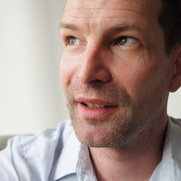
\includegraphics[width=0.3\textwidth]{images/Matthias_Schlossberger.png}
%	\caption{Matthias Schlo"sberger}
%	\label{fig:MS}
%\end{figure}


%\begin{figure}[h]
%	\centering
%	
\includegraphics[width=0.5\textwidth]{images/template.png}
%	\caption{Template Bild}
%	\label{fig:template}
%\end{figure}

\end{document}
